 \documentclass[a4paper,10pt,conference]{ieeeconf}

\IEEEoverridecommandlockouts
\overrideIEEEmargins

\usepackage{cite}
\usepackage{amsmath,amssymb,amsfonts}
\usepackage{graphicx}
\usepackage{textcomp}
\usepackage{xcolor}
\usepackage{booktabs}
\usepackage{array}
\usepackage{url}
\usepackage{stfloats}
\usepackage[hidelinks]{hyperref}

\graphicspath{{Figures/}}


\title{\LARGE \bf
Body-Motion Control of a Simulated Aerial Swarm from a First-Person View}

\author{
\authorblockN{
Yang Chen$^{\dagger}$,
Darius Giannoli$^{\dagger}$, and
Dario Floreano,
\IEEEmembership{Fellow, IEEE}
}
\thanks{$^{\dagger}$Y. Chen and D. Giannoli contributed equally to this work.}%
\thanks{All authors are with the Laboratory of Intelligent Systems,
\'{E}cole polytechnique f\'{e}d\'{e}rale de Lausanne (EPFL),
Lausanne, Switzerland (e-mail: chenyang@ai.iit.tsukuba.ac.jp;
darius.giannoli@epfl.ch; dario.floreano@epfl.ch).}%
\thanks{Videos are available in the
\protect\href{https://www.youtube.com/playlist?list=PLTn4QPxGFMEU}
{online video playlist}.}%
\thanks{This work was supported by the Swiss National Science Foundation
under Grant 200020\_212077.}%
\thanks{This study involving human participants was approved by the EPFL
Human Research Ethics Committee under Application No.\ HREC 092-2023.}%
}

\begin{document}

\maketitle
\thispagestyle{empty}
\pagestyle{empty}



\begin{abstract}

Immersive first-person-view teleoperation of aerial swarms requires concurrent
control of collective motion, view direction, and formation size. We developed
a participant-calibrated upper-body interface providing five-DOF control
through torso, controller, and head motion. In a within-subject study, 14
participants navigated a simulated 15-agent swarm through three-dimensional
obstacle courses using the implemented body-motion interface and a conventional transmitter. the implemented body-motion interface
reduced completion time by 19.4\% and centroid path length by 7.0\%, produced
more direct trajectories, yielded 88.8\% lower delivered-command variation, and
increased multi-DOF coordination by 22.5 percentage points. No clear
differences were detected in gate-centering error, collection yield, crash and
disconnection counts, overall workload, or usability, while physical demand was
higher with the implemented body-motion interface for all participants. These results indicate an
efficiency advantage for an upper-body interface that distributes concurrently
varying command dimensions across separate body segments.
\end{abstract}


% =====================================================================
\section{Introduction}

\section{Introduction}

Aerial swarms can extend sensing and coverage by coordinating many robots, but
missions that depend on human judgment still require an effective interface
between one operator and the collective
\cite{kolling2016survey,hocraffer2017meta}. Rather than command individual
agents, the operator can steer the swarm through a smaller set of collective
commands. In three-dimensional environments, however, several commands may
need to change concurrently. Passing through an opening can require simultaneous
adjustment of planar translation, altitude, formation spacing, and view
direction. The interface must therefore support coordinated control of multiple
continuous degrees of freedom (DOF), rather than forcing the operator to make
these adjustments sequentially.

This control problem is affected by how the swarm is viewed. A top-down view
(TDV) provides an external overview that makes the swarm's global state,
including its spatial extent, connectivity, and relationship to surrounding
obstacles, directly visible. Producing this view in an uninstrumented
environment may nevertheless require external infrastructure, a dedicated
viewing platform, or real-time scene reconstruction. A dedicated viewing agent
can also introduce a single point of failure into an otherwise distributed
system. A first-person view (FPV) can instead be streamed from a \emph{focal
agent}, defined here as the swarm member whose onboard camera currently supplies
the operator's view. The camera source can be transferred if that agent becomes
unavailable, preserving the distributed character of the swarm
\cite{ben_focaldrone}. The trade-off is that the camera's limited field of view
and occlusions hide much of the swarm and environment. Moreover, the viewpoint
moves with the focal agent, its reference frame rotates with the view, and the
feed may transfer between agents. FPV therefore restricts global awareness
precisely while the operator must coordinate several swarm DOF.

\begin{figure}[!t]
\centering
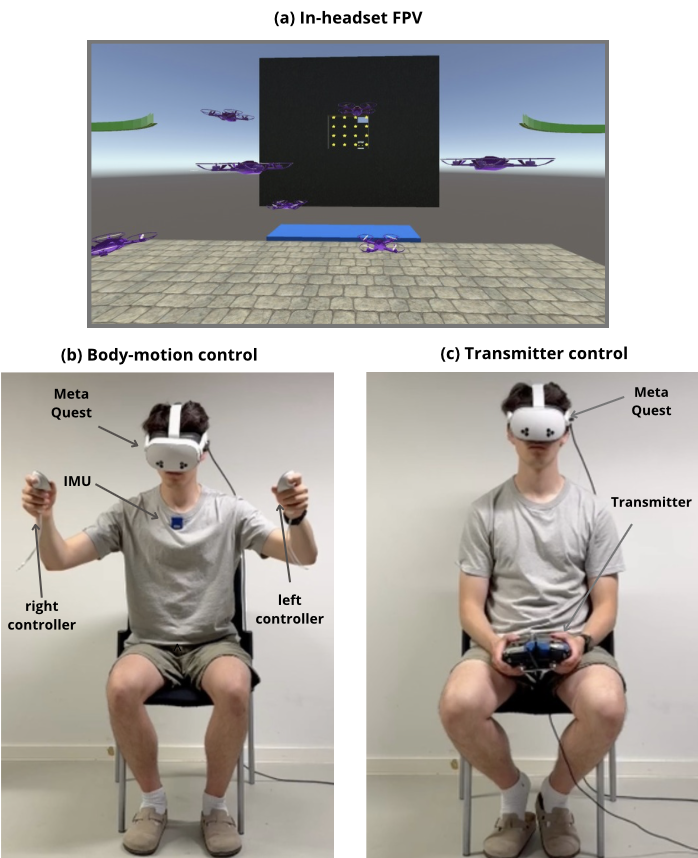
\includegraphics[width=\columnwidth]{Figures/111.png}
\caption{Experimental interfaces and common visual feedback:
(a) the in-headset rear-focal FPV view, (b) body-motion control using
a torso-mounted IMU and hand controllers, and (c) transmitter control.
Both conditions used the same headset, visual feedback, and swarm
command space.}
\label{fig:study_overview}
\end{figure}

Jarvis et al.\ demonstrated that a rear-focal FPV can support one-to-many swarm
teleoperation and compared different placements and combinations of onboard
views \cite{ben_focaldrone}. Their interface assigned planar translation,
vertical motion, view yaw, and formation spacing to two transmitter sticks and
a rotary control. This established the feasibility of focal-agent FPV, but left
an interaction problem unresolved: whether a conventional handheld transmitter
is well matched to a task requiring concurrent adjustment of five continuous
DOF. Multidimensional-input research distinguishes separable control, in which
dimensions tend to be adjusted independently, from integral control, in which
several dimensions can be varied together
\cite{jacob1994integrality,zhai1998quantifying}. In this setting, the allocation
of several commands across thumbsticks and a separate rotary control may become
a bottleneck during maneuvers that require simultaneous translation, altitude,
spacing, and viewpoint changes.

Upper-body motion offers a different allocation of these commands. Head, torso,
and hand movements provide several continuous input dimensions that can be
assigned to distinct swarm DOF while retaining spatial correspondence between
body motion and commanded motion. Body--machine interfaces have already enabled
immersive and personalized control of individual drones
\cite{rognon2018flyjacket,miehlbradt2018datadriven,
macchini2024datadriven}. Importantly, Macchini et al.\ found that robots with
more DOF elicited the use of more body segments and greater variation in motion
strategies across users, increasing the need for personalized mappings
\cite{macchini2024datadriven}. This result motivates a participant-calibrated
interface for the present five-DOF task. At swarm level, personalized hand
motion has supported four-dimensional control from an external viewpoint
\cite{macchini2021personalized}, while tactile and gesture-based systems have
supported other forms of swarm and formation control
\cite{tsykunov2019swarmtouch,kratky2025gesture}. Together, these studies suggest
that body motion can support multidimensional control, but do not establish
whether it remains effective when the operator acts through a moving
focal-agent FPV.

We therefore investigate whether distributing five continuous swarm commands
across the head, torso, and hands can address the input bottleneck of
focal-agent FPV teleoperation. We implement a participant-calibrated interface
in which torso inclination commands planar velocity, mean hand height commands
vertical velocity, hand separation commands formation spacing, and head yaw
commands FPV yaw rate. We compare the complete interface with a conventional
radio-control transmitter in a within-subject study of 14 participants
navigating a simulated swarm through three-dimensional obstacle courses. The
contributions are (i) a five-DOF upper-body mapping that remains aligned with
the focal agent's reference frame during view rotation and transfer, and
(ii) an experimental comparison characterizing traversal efficiency,
trajectory geometry, control behavior, task accuracy, swarm integrity,
workload, usability, and preference.






\section{Swarm Control System and Input Interfaces}
% --- 2a. Methodology: the interface and the body-to-swarm mapping ---

\subsection{Shared Swarm and FPV System}
\label{sec:system}

Both input conditions generated a common five-dimensional command vector for
the simulated 15-agent swarm:
\begin{equation}
\mathbf{u}_t =
\left[
v_{\mathrm{fwd},t}^{\mathrm{ref}},
v_{\mathrm{lat},t}^{\mathrm{ref}},
v_{\mathrm{vert},t}^{\mathrm{ref}},
\dot{\psi}_{t}^{\mathrm{cmd}},
\rho_t^{*}
\right]^{\mathsf T}.
\label{eq:swarm_command}
\end{equation}
The first three components specify focal-frame horizontal and world-vertical
reference velocities, $\dot{\psi}_{t}^{\mathrm{cmd}}$ specifies FPV yaw rate,
and $\rho_t^{*}$ specifies target agent spacing.


A decentralized Olfati--Saber controller~\cite{olfatisaber2006flocking}
combined clearance regulation, velocity alignment, reference-velocity
tracking, and obstacle repulsion. At 50 Hz, surviving agents were represented as vertices of an undirected interaction graph. An edge connected agents \(i\) and \(j\) when their Euclidean separation was less than \(R_t=\max(2\rho_t^{*},\,\rho_t^{*}+2~\mathrm{m})\), where \(\rho_t^{*}\) was the commanded surface-to-surface clearance. Connected components were computed from this graph, and surviving agents outside the largest connected component were classified as disconnected.

We fixed the visual interface to a rear-focal FPV rather than treating
viewpoint as an additional experimental factor. A camera on the rearmost agent
places most of the controlled swarm ahead of the camera and therefore within
its forward field of view. Moreover, Jarvis et al.\ found that rear-of-swarm
views were preferred and supported more precise flight, fewer crashes, and
lower workload than front-of-swarm views, whereas presenting multiple views
simultaneously increased completion time \cite{ben_focaldrone}. Because the
present study investigates the input interface rather than viewpoint
selection, we adopted this evidence-supported single-view configuration and
held it constant across both conditions.

Following the focal-agent selection method of Jarvis et
al.~\cite{ben_focaldrone}, the agent furthest back in the horizontal viewing
direction provided the stereoscopic FPV. The system switched to a new agent
only if it remained at least 0.5~m further back for 0.5~s.

In both conditions, participants used a virtual reality (VR) headset (Meta Quest 3S, Meta, USA) to view the FPV. Three devices measured the implemented body-motion interface. The headset measured head yaw. Two handheld controllers measured 3D hand positions. A chest-mounted inertial measurement unit (LPMS-B2, LP-Research, Japan) measured torso inclination. The swarm controller, command limits, focal-agent logic, and simulation were the same for both conditions. Only the input hardware and filtering differed.

\subsection{Body-to-Swarm Mapping}
\label{sec:mapping}

At time $t$, the interface measured sagittal and lateral torso inclination
$(\theta_t,\phi_t)$, headset yaw $\psi_t$, mean controller height
\[
h_t=\frac{y^W_{L,t}+y^W_{R,t}}{2},
\]
and controller separation
\[
s_t=\left\lVert\mathbf{p}^W_{R,t}-\mathbf{p}^W_{L,t}\right\rVert .
\]
Translation and yaw used rate control, meaning a sustained posture produced continuous motion. In contrast, controller separation mapped directly to the desired formation clearance.

\emph{Participant-specific normalization:}
Each rate-controlled signal was mapped to $[-1,1]$ using its calibrated lower
extreme, neutral value, and upper extreme $(q^{-},q^{0},q^{+})$, with a
deadzone of half-width $d$ around neutral. Let
$q_{\mathrm{L}}=q^{0}-d$ and $q_{\mathrm{U}}=q^{0}+d$. The normalization was
\begin{equation}
\mathcal{D}(q_t;q^{-},q^{0},q^{+},d)=
\begin{cases}
\displaystyle
\max\!\left(-1,
\frac{q_t-q_{\mathrm{L}}}{q_{\mathrm{L}}-q^{-}}\right),
& q_t<q_{\mathrm{L}},\\[6pt]
0,
& q_{\mathrm{L}}\leq q_t\leq q_{\mathrm{U}},\\[3pt]
\displaystyle
\min\!\left(1,
\frac{q_t-q_{\mathrm{U}}}{q^{+}-q_{\mathrm{U}}}\right),
& q_t>q_{\mathrm{U}}.
\end{cases}
\label{eq:deadzone_mapping}
\end{equation}
Separate scaling on either side of neutral accommodated asymmetric ranges of
motion.





\emph{Translation:}
The normalized translation commands were
\begin{align}
c_{\mathrm{fwd},t}
&=\mathcal{D}(\theta_t;\theta^{-},0,\theta^{+},5^{\circ}),
\nonumber\\
c_{\mathrm{lat},t}
&=\mathcal{D}(\phi_t;\phi^{-},0,\phi^{+},5^{\circ}),
\nonumber\\
c_{\mathrm{vert},t}
&=\mathcal{D}(h_t;h_{\min},h_0,h_{\max},0.05~\mathrm{m}).
\label{eq:body_rate_commands}
\end{align}
Positive commands denoted forward, rightward, and upward motion. The normalized
commands were smoothed, with the resulting values denoted by
$(\bar c_{\mathrm{fwd},t},\bar c_{\mathrm{lat},t},
\bar c_{\mathrm{vert},t})$. These values were then scaled by
$10~\mathrm{m\,s^{-1}}$ to obtain the corresponding reference velocities
$(v_{\mathrm{fwd},t}^{\mathrm{ref}},v_{\mathrm{lat},t}^{\mathrm{ref}},
v_{\mathrm{vert},t}^{\mathrm{ref}})$ in Eq.~\eqref{eq:swarm_command}.

% The forward and lateral velocities were defined relative to the displayed
% heading and updated after FPV rotation or viewpoint transfer.

\emph{Inter-agent spacing:} 
The system mapped the controller separation $s_t$ linearly from the participant-specific range $[s_{\min},s_{\max}]$ to a target surface-to-surface clearance $\rho_t\in[1,5]~\mathrm{m}$. The system clipped this mapping at the calibrated limits and smoothed it, produc the applied command $\rho_t^*$ in Eq.~\eqref{eq:swarm_command}.

\emph{FPV yaw:}
With
$\Delta\psi_t=
\operatorname{wrap}_{[-180^{\circ},180^{\circ})}
(\psi_t-\psi_{0,t})$
denoting the head-yaw deviation from its neutral orientation, the FPV yaw-rate
command was
\begin{equation}
\dot{\psi}^{\,\mathrm{cmd}}_t
=
48^{\circ}\mathrm{s}^{-1}
\mathcal{D}\!\left(
\Delta\psi_t;\psi_{\mathrm{L}},0,\psi_{\mathrm{R}},10^{\circ}
\right).
\label{eq:yaw_rate}
\end{equation}
Returning the head to neutral stopped FPV rotation without restoring the
previous viewing direction.
All parameters were selected through pilot and informal testing.


\begin{figure*}[!t]
\centering
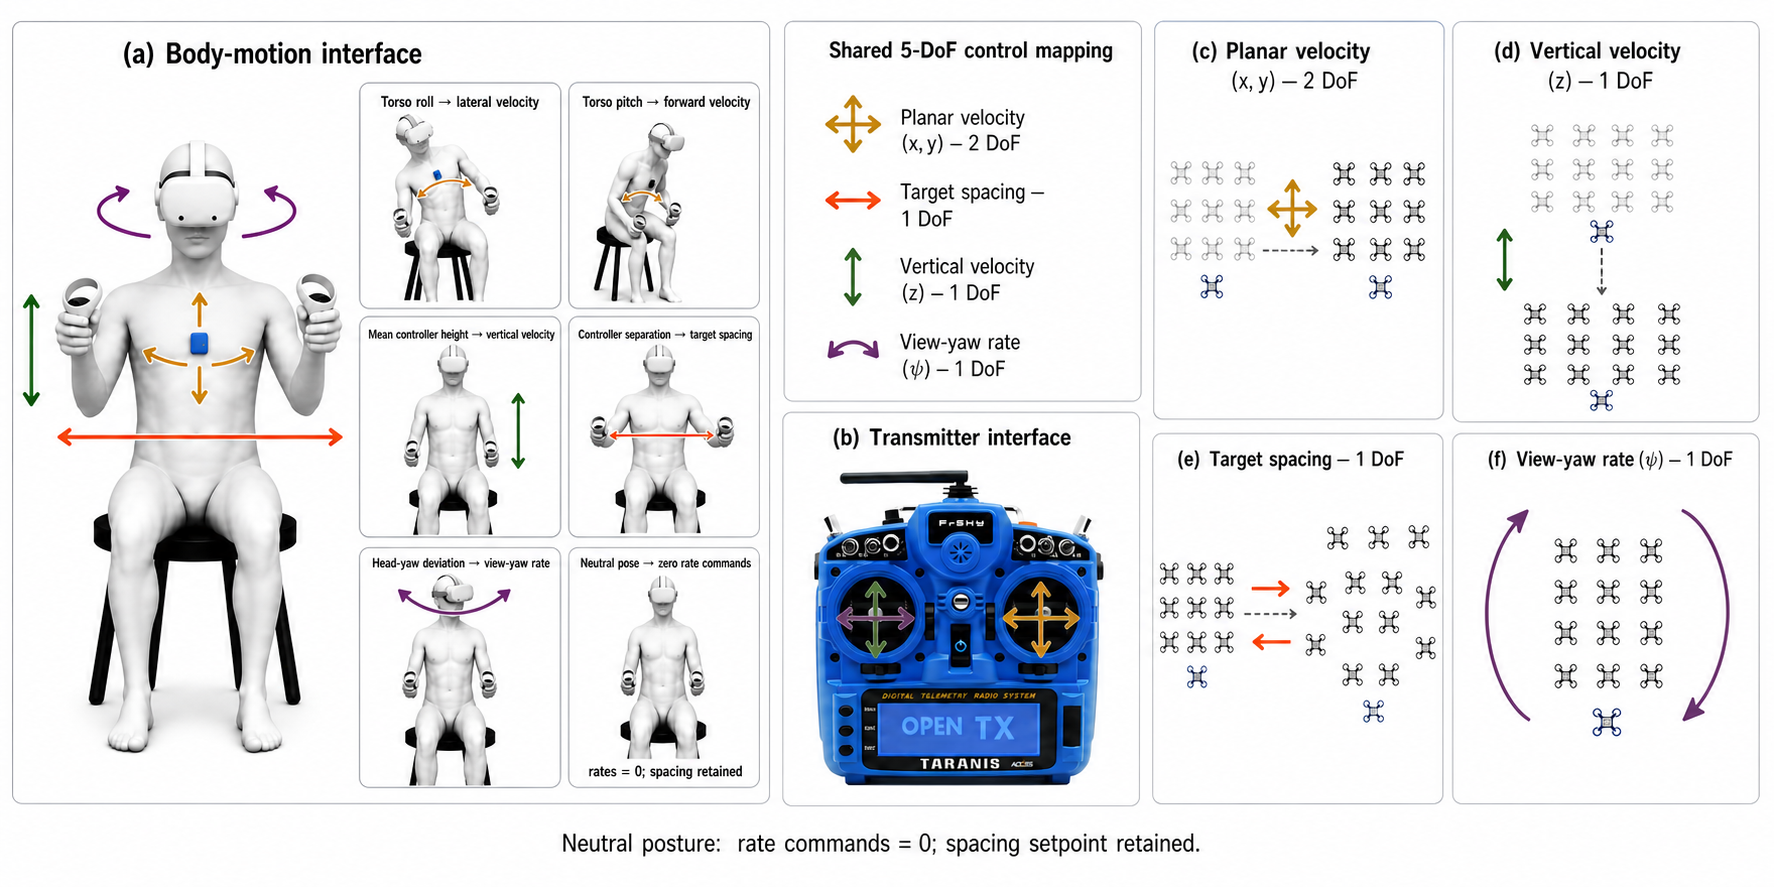
\includegraphics[width=\textwidth]{Figures/l.png}
\caption{Body-to-swarm control mappings. Subfigures (a)--(e) illustrate how the participant's posture and hand positions map to specific swarm commands. The neutral pose (f) halts all movement but maintains the current spacing setpoint. Faded formations indicate the direction of the commanded motion, scaling, or view rotation.}
\label{fig:mapping}
\end{figure*}


\subsection{Participant-Specific Calibration}
\label{sec:calibration}
Each participant completed a one-time guided 13-pose calibration to record
seated neutral postures and comfortable motion limits. The chair configuration and Quest tracking origin remained fixed thereafter.

Calibration included five torso poses (neutral and maximum forward, backward,
left, and right), three head-yaw poses (neutral and maximum left and right),
two controller-separation poses (minimum and maximum), and three
controller-height poses (minimum, neutral, and maximum). Neutral torso and head
poses defined the IMU orientation offset and headset yaw reference $\psi_0$,
respectively; only $(s_{\min},s_{\max})$ parameterized the absolute spacing
mapping.

The measured bounds directly parameterized the translation, yaw-rate, and
spacing mappings.
Table~\ref{tab:calibration_summary} summarizes the resulting spans; angular
spans combine opposing excursions, whereas position spans are
maximum--minimum differences.

\begin{table}[b]
\centering
\caption{Calibrated input spans across participants ($N=14$).}
\label{tab:calibration_summary}
\footnotesize
\setlength{\tabcolsep}{3.5pt}
\begin{tabular}{@{}lcc@{}}
\toprule
Input span & Mean $\pm$ SD & Range \\
\midrule
Sagittal torso ($^\circ$)       & $56.4 \pm 18.4$  & $34.2$--$98.1$ \\
Lateral torso ($^\circ$)        & $52.0 \pm 18.0$  & $26.2$--$81.2$ \\
Head yaw ($^\circ$)             & $117.5 \pm 24.7$ & $65.6$--$138.0$ \\
Controller separation (m)       & $1.10 \pm 0.33$  & $0.70$--$1.51$ \\
Controller height (m)           & $0.77 \pm 0.22$  & $0.43$--$1.22$ \\
\bottomrule
\end{tabular}
\end{table}

\subsection{Transmitter Baseline}
\label{sec:transmitter}

A conventional radio-control transmitter (Taranis X9D Plus, FrSky, China) generated the same command vector, $\mathbf{u}_t$, as the body-motion interface. As shown in Fig. ~\ref{fig:study_overview}, the right stick controlled planar
velocity, the left horizontal axis controlled FPV yaw rate, the
non-self-centering left throttle controlled vertical velocity, and the right
rotary knob set target inter-agent clearance. Stick axes used a symmetric
deadzone, while the knob mapped linearly
to $\rho^*\in[1,5]$~m. The transmitter received no participant-specific
calibration or additional temporal filtering.

% =====================================================================

\label{sec:experiment}

\section{Experimental Evaluation}
\label{sec:experiment}


\subsection{Participants and Study Design}
\label{sec:participants_design}

The study included $N=14$ adults recruited from the local university
community (10 men and 4 women; age: $22.4 \pm 4.0$ years, range 19--35).
Eligibility required self-reported ability to perform the seated
upper-body movements and vision compatible with the VR headset. All
participants completed the study, provided written informed consent, and were
compensated.

A two-condition within-subject design compared the body-motion and transmitter interfaces described in Sections~\ref{sec:system}--\ref{sec:transmitter}. The
first participant's starting interface was selected at random and alternated
thereafter, yielding seven participants per sequence. Both conditions were
completed while seated during a single session lasting approximately 1~h.

\subsection{Task and Procedure}
\label{sec:task}



All participants received identical prerecorded instructions and
demonstrations. They were asked to complete each course as quickly as possible while passing near the opening centers, collecting stars, and minimizing crashes and disconnections. Participants viewed only stereoscopic FPV, with no timer, score, or task-status display.

Each recorded course contained seven gates whose positions, heights, and
opening sizes were varied to require horizontal translation, altitude
adjustment, and formation-spacing control. The 90-degree turn additionally
required participants to rotate the FPV and continue navigating in the rotated
focal-agent reference frame. Collectible stars were distributed across the
gate openings to encourage participants to control the spatial extent of the
swarm rather than merely guide the focal agent or swarm centroid through each
gate. Collection yield therefore provided a secondary measure of collective
task performance.

A star was collected when any agent entered its trigger; wall or inter-agent collisions removed the affected agent, and survivors outside the largest connected component were classified as disconnected at each sample.


The courses were designed to compare the two interfaces under identical, repeatable conditions rather than to evaluate directional symmetry. Consequently, only one direction of 90° turning was represented. Although both interfaces were evaluated on the same courses, the results do not establish that performance would be unchanged for opposite-direction or repeated turns. Future studies should use mirrored or direction-counterbalanced courses.


Before the body-motion block, participants completed the calibration described
in Section~\ref{sec:calibration}. Each interface block began with familiarization
on the practice course: participants first maneuvered freely with standardized
experimenter guidance and then completed one unrecorded full-course traversal.
Two recorded runs followed in fixed order.



After each interface block, participants completed the weighted NASA Task Load
Index (NASA-TLX)~\cite{hart1988nasatlx} and the System Usability Scale
(SUS)~\cite{brooke1996sus}, referring only to the two recorded runs. After both
blocks, they reported interface preference and relative motion sickness and could provide optional
free-text comments.

\begin{figure}[b]
\centering
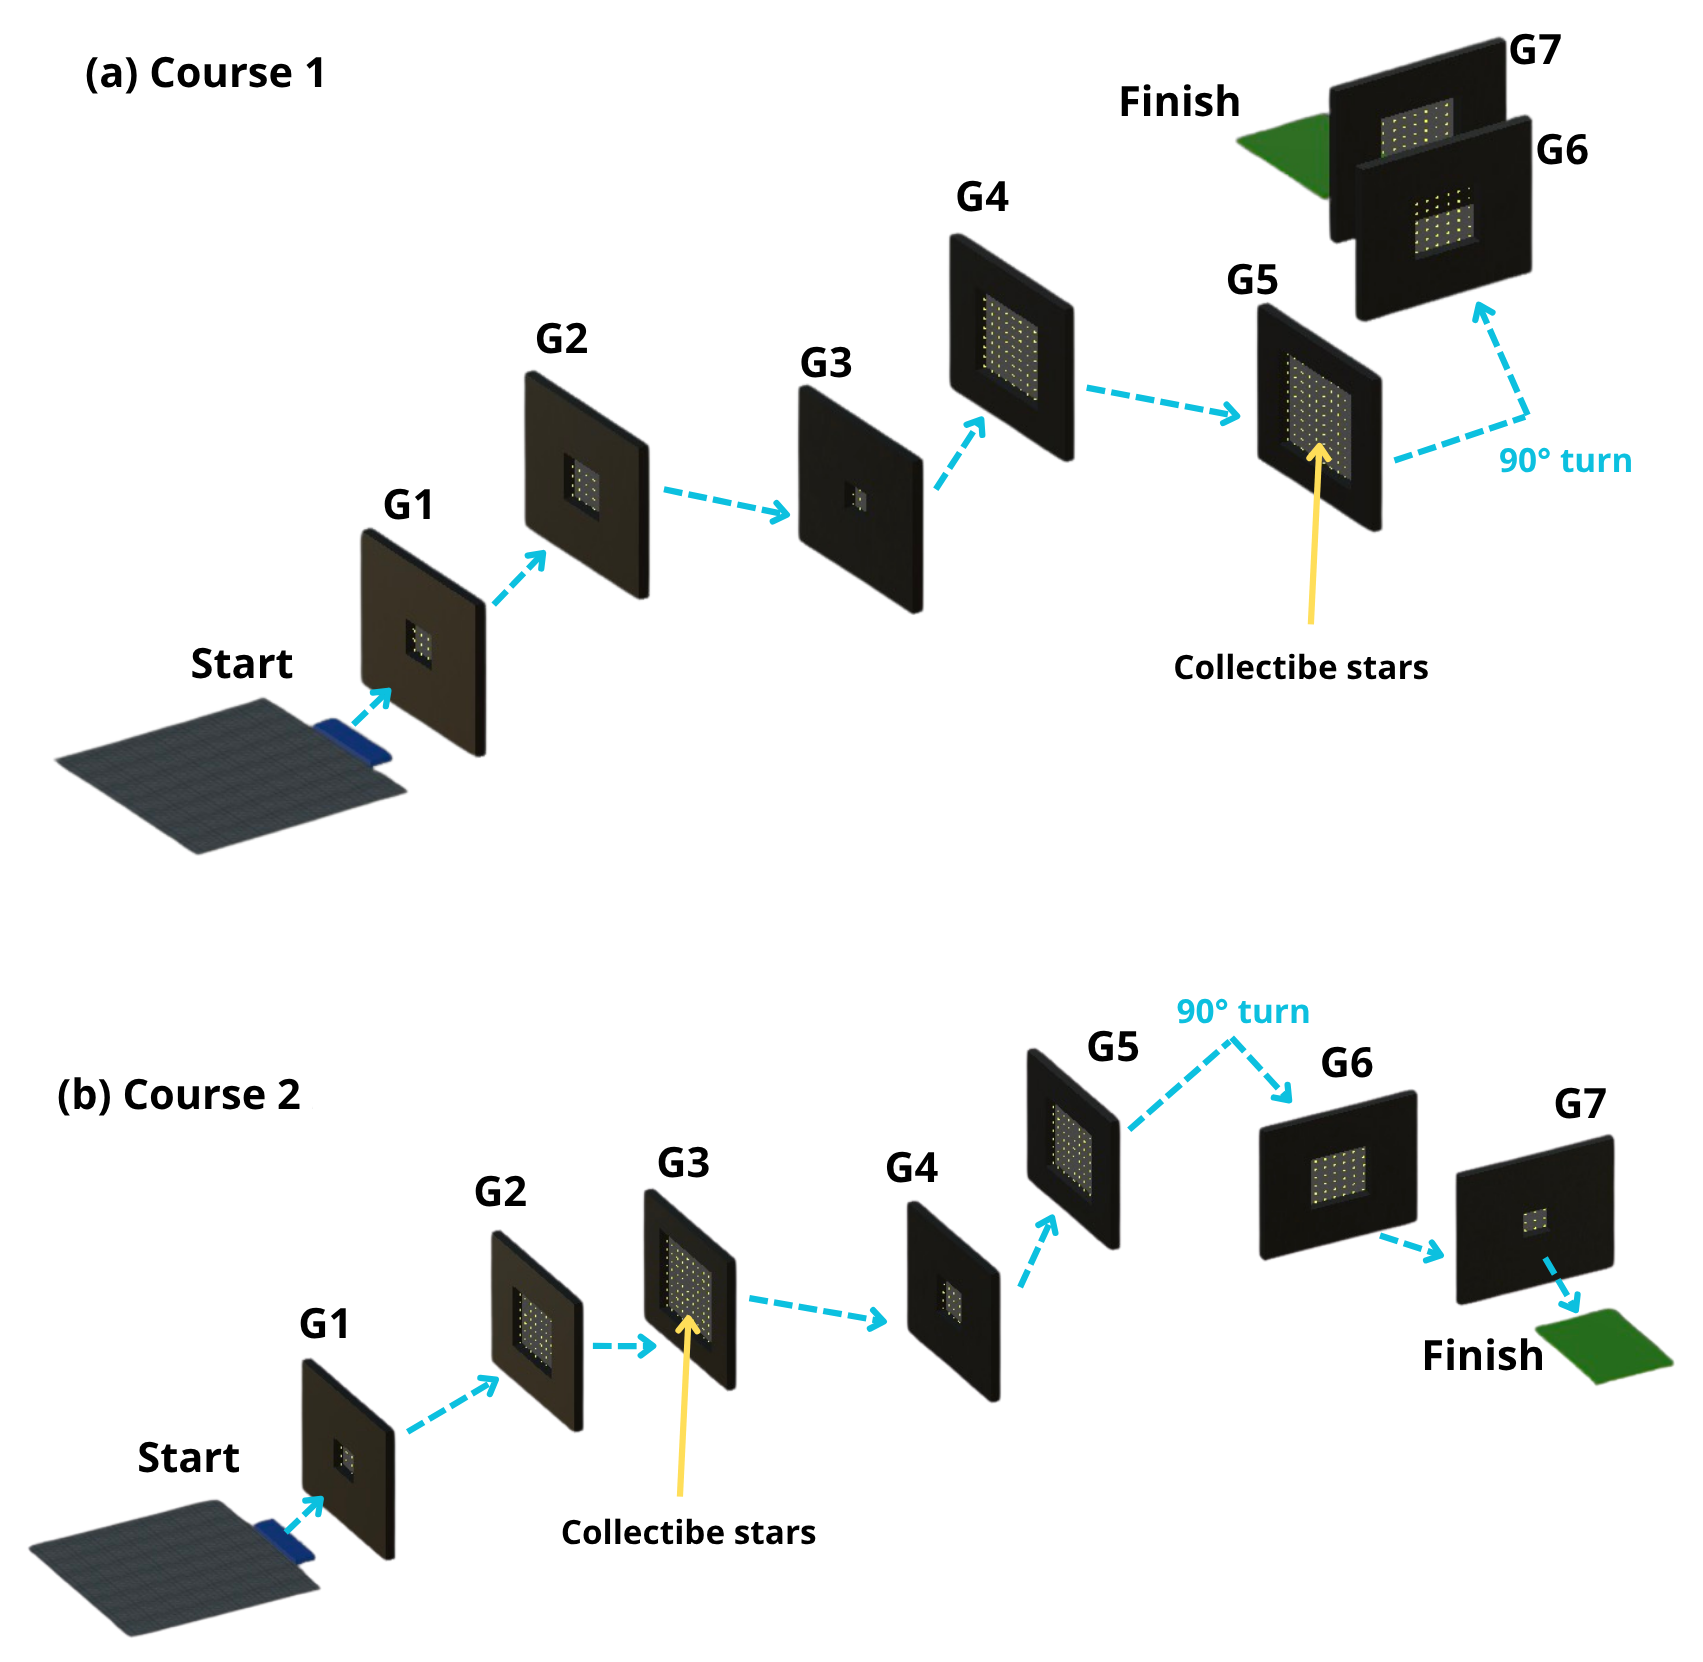
\includegraphics[width=\columnwidth]{Figures/layouts.png}
\caption{Both obstacle course layouts.
Labels G1--G7 mark the gate sequence; dashed arrows show traversal direction.}
\label{fig:course_layouts}
\end{figure}


\subsection{Evaluation Metrics}

Completion time was the primary outcome, consistent with task-oriented HRI
evaluation~\cite{steinfeld2006metrics}. Other measures described trajectory
characteristics, task performance, swarm integrity, delivered commands, and
subjective experience.

\emph{Traversal efficiency.}
Completion time $T$ was measured from the recorded start event to the finish
event. The centroid path length L was the total 3D distance traveled by the controlled-component centroid. The mean speed was $\bar v=L/T$. Because both metrics relate to completion time, we treat them as supporting outcomes.


\emph{Trajectory characteristics.}
Path directness used
the endpoint-distance-to-path-length definition of path
efficiency~\cite{mavrogiannis2022socialmomentum}:
\begin{equation}
D_{\mathrm{path}}
=
\frac{1}{L}
\sum_{j=1}^{8}
\left\|
\mathbf{x}_{j,\mathrm{end}}
-
\mathbf{x}_{j,\mathrm{start}}
\right\|_2.
\label{eq:path_directness}
\end{equation}
The eight segments covered the path from the start to the first gate, between
gates, and from the final gate to the finish. The calculation used the measured
segment endpoints.

For each segment, excess horizontal travel $H_{\mathrm{exc}}$ was the
horizontal path length in the $x$--$z$ plane minus the direct horizontal
displacement between its endpoints. Excess vertical travel
$V_{\mathrm{exc}}$ was the total absolute height change minus the direct
height change. Both measures were summed across the eight segments. Lower
excess travel indicates fewer unnecessary horizontal detours or vertical
movements.

\emph{Gate-centering error.} For each gate we linearly interpolate the swarm
centroid to the instant it crosses the gate plane and measure its offsets from
the gate center within that plane: $d_h$ along the gate's horizontal axis and
$d_v$ vertically. We report the in-plane distance $\sqrt{d_h^2+d_v^2}$ averaged
over the $N_g=7$ gates, so that lower values indicate crossings closer to the
gate center.

Collection yield was the fraction of the 316 available stars collected.
Crash count was the number of agents that crashed during a run.
Disconnection count was the number of agent-disconnection events recorded
during a run.

\emph{Delivered-command behavior.}
Each command was normalized to $[0,1]$. Let $\mathbf{q}_k$ denote the five commands at sample $k$, and let $\tau=t_M-t_1$ represent the total duration. The delivered-command variation was
\begin{equation}
E_{\mathrm{cmd}} = \frac{\tau}{5} \sum_{k=1}^{M-1} \frac{\lVert\mathbf{q}_{k+1}-\mathbf{q}_k\rVert_2^2} {t_{k+1}-t_k}.
\label{eq:command_metrics}
\end{equation}
Lower values indicate less variation in the delivered commands.

\emph{Multi-DOF coordination.}
We measured multi-DOF coordination as the percentage of active control time
during which at least two of the five commands changed simultaneously. A
command was considered changing when its normalized change rate exceeded
$0.10~\mathrm{s^{-1}}$. Active control time comprised intervals in which at
least one command's normalized change rate exceeded this threshold. Higher
values indicate more simultaneous use of multiple command dimensions. 
% Because the tested interfaces applied different online filters, both measures characterize the delivered-command pipelines rather than the input hardware or participants' unfiltered movements.

% =====================================================================
\section{Results}

All 56 runs were retained; the two runs per interface were averaged for each
participant, yielding 14 paired observations. Interfaces were compared using exact two-sided Wilcoxon signed-rank tests ($\alpha=0.05$)~\cite{wilcoxon1945ranking}, with Holm adjustment within outcome families~\cite{holm1979procedure}.

Figure 4 shows the statistical distributions for all evaluated performance and subjective metrics.

\begin{figure*}[t]
\centering
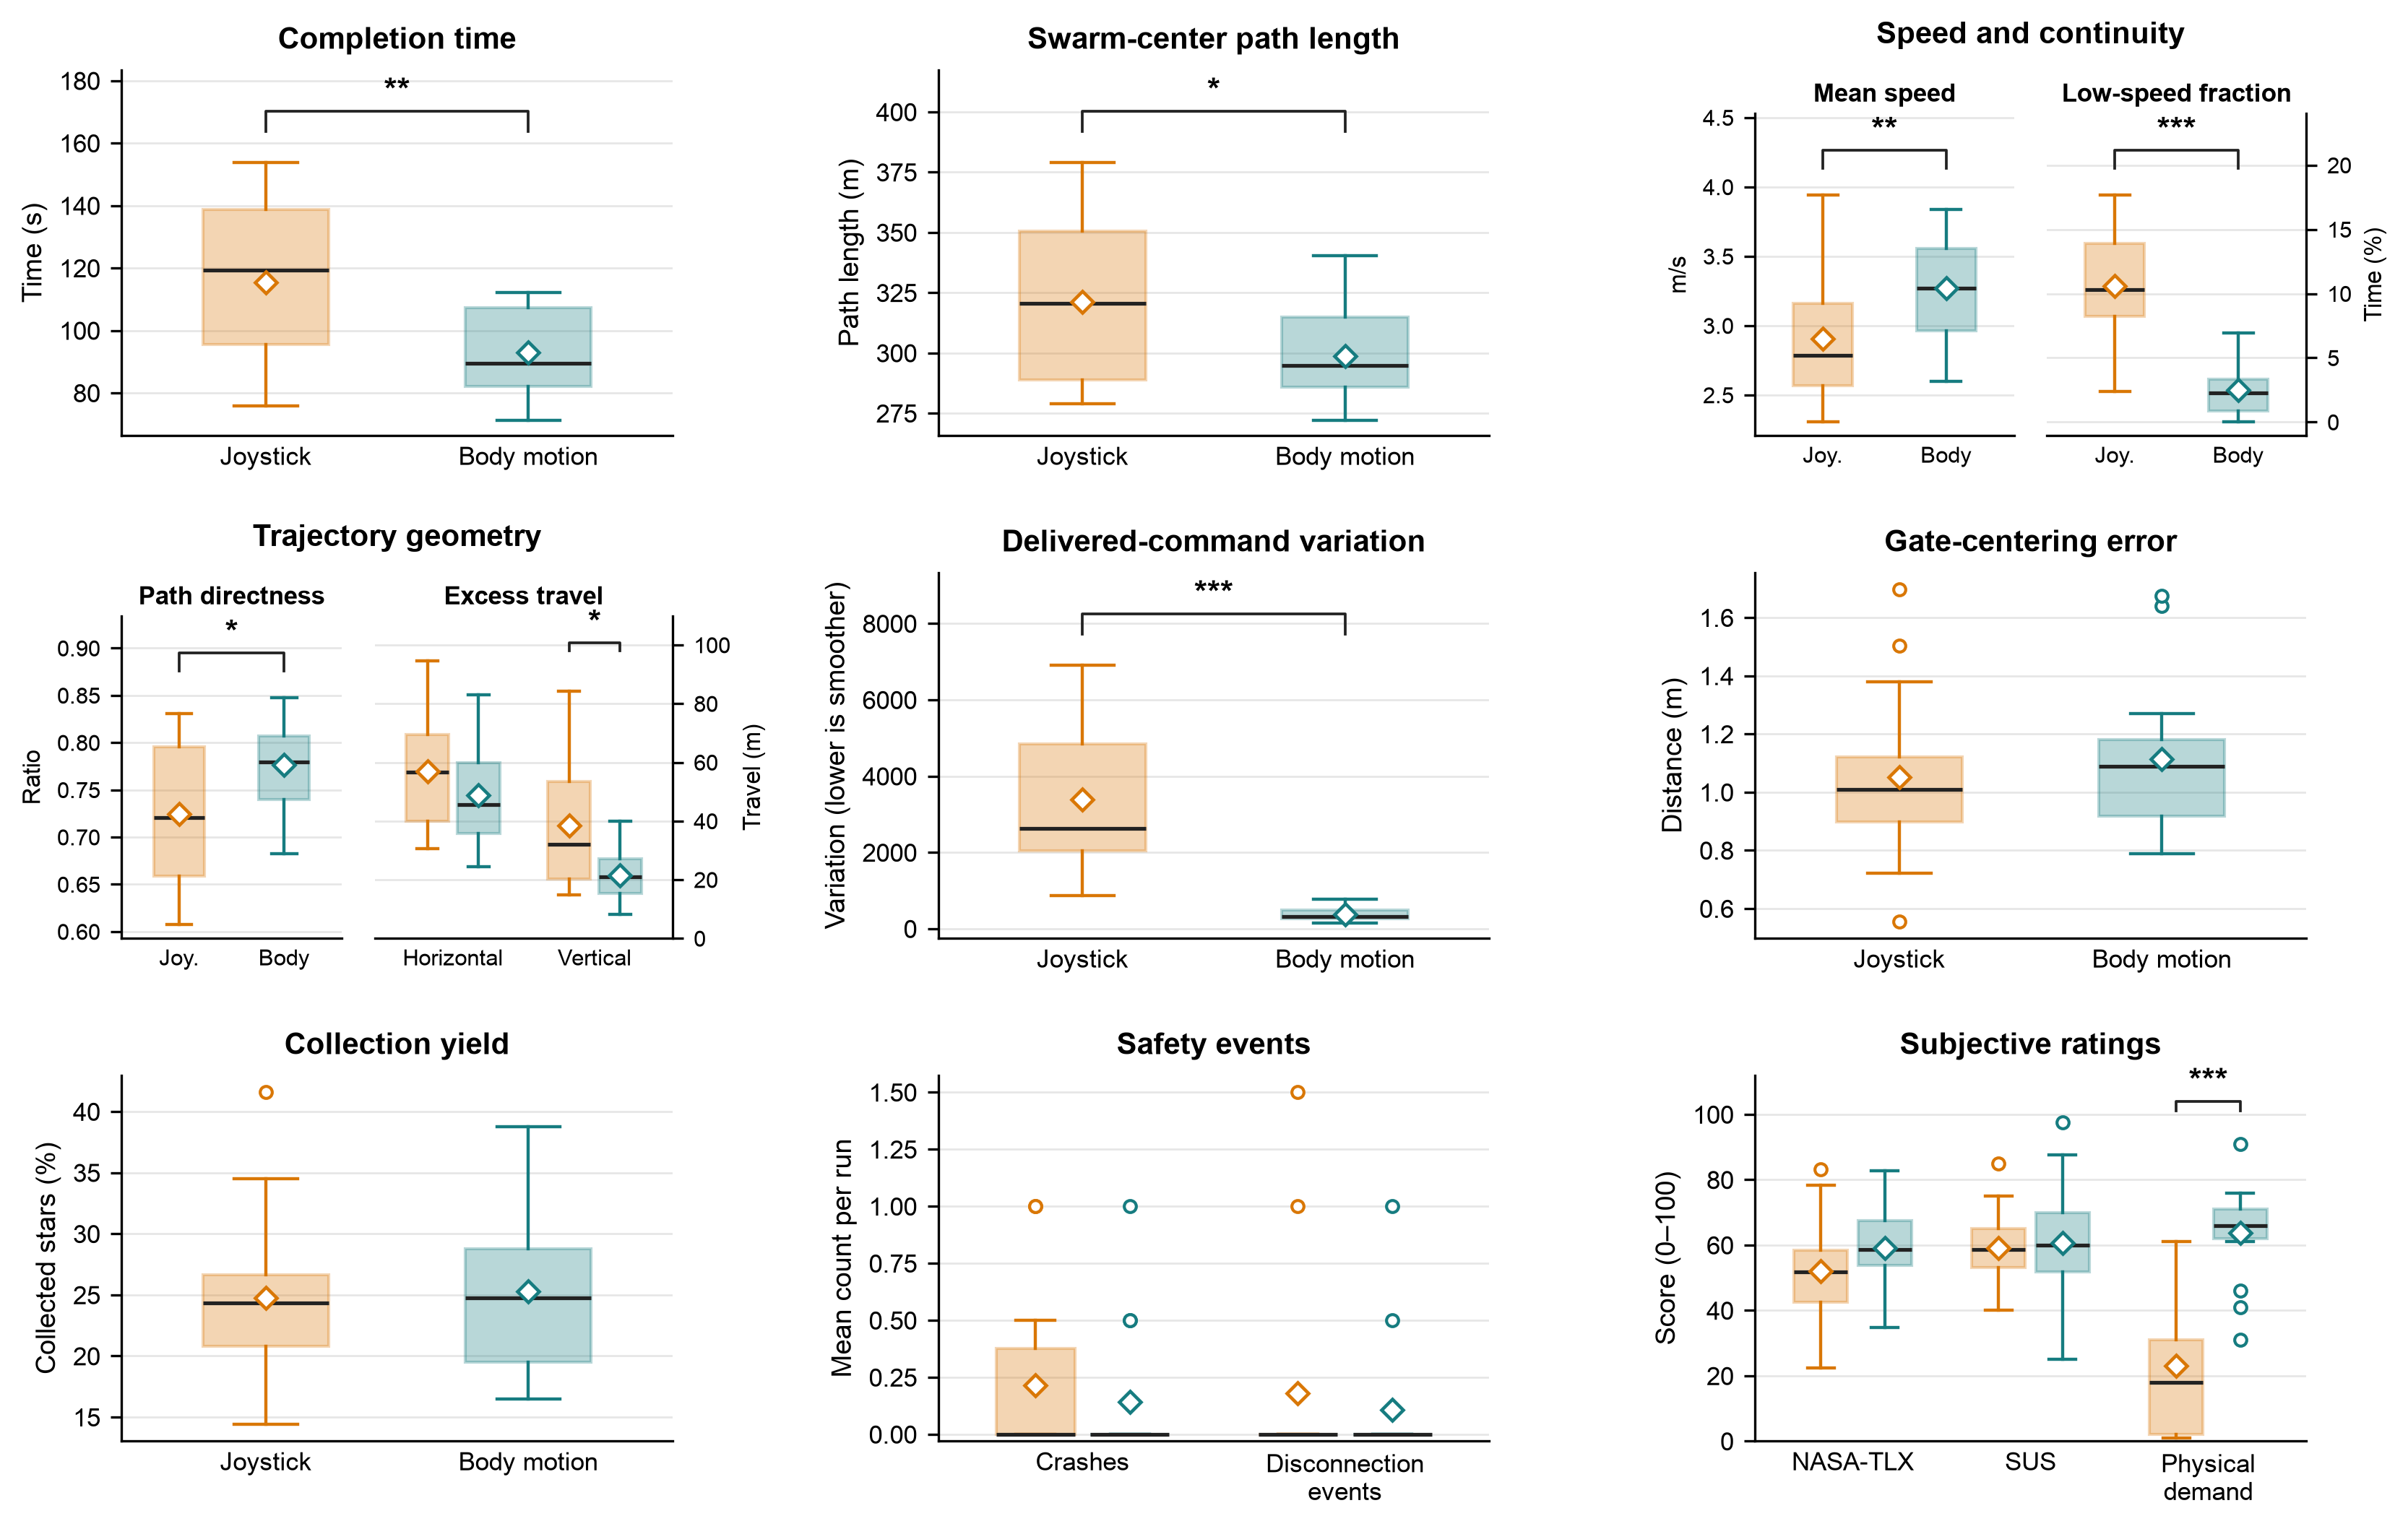
\includegraphics[width=\textwidth]{Figures/box.png}
\caption{Participant-level outcomes for transmitter and body-motion control
($n=14$). 
% Delivered-command variation and multi-DOF coordination are shown for the recorded pipelines.
Boxes show interquartile ranges with median lines; diamonds indicate means
and circles indicate outliers. Orange denotes transmitter and teal denotes body
motion. Stars mark Holm-adjusted paired comparisons
($*p<0.05$, $**p<0.01$, $***p<0.001$).}
\label{fig:paired_results}
\end{figure*}

\emph{Traversal efficiency.} the implemented body-motion interface significantly improved all traversal metrics compared to the transmitter. Completion time decreased by 19.4\%, representing a mean reduction of 22.4~s (Holm-adjusted $p=0.001$) with 13 of the 14 participants going faster using the implemented body-motion interface. Centroid path length was 7.0\% shorter (Holm-adjusted $p=0.011$), and mean speed was 12.5\% higher (Holm-adjusted $p=0.001$).

\emph{Trajectory characteristics.}
the implemented body-motion interface produced more direct trajectories than the
transmitter. Path directness increased by 0.052
(Holm-adjusted $p=0.032$). Excess vertical
travel decreased by 44.0\%, corresponding to 16.9~m
(Holm-adjusted $p=0.049$) while excess horizontal
travel was 14.2\% lower with the implemented body-motion interface (48.8 versus 56.8~m), but the
difference was not statistically detectable (mean difference $-8.0$~m,
Holm-adjusted $p=0.153$).
Figure~\ref{fig:trajectory_overlays} illustrates these trajectory
characteristics.

\begin{figure}[!b]
\centering
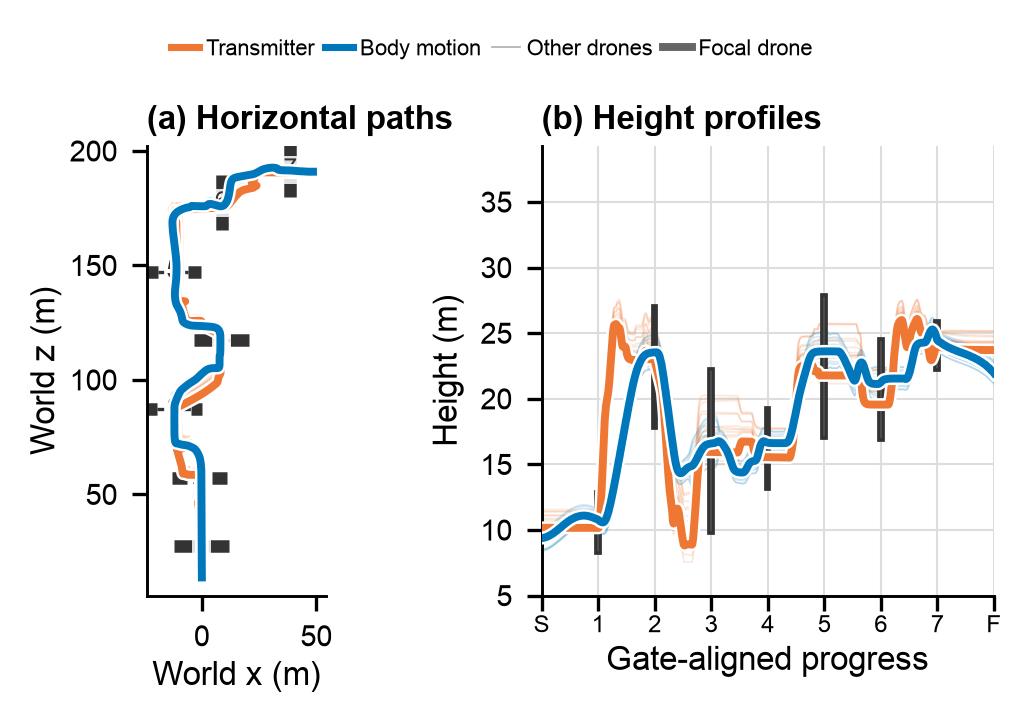
\includegraphics[width=\columnwidth]
{Figures/a.png}
\caption{Course 2 individual-drone trajectories for one participant: (a) horizontal paths and (b) gate-aligned height profiles under transmitter and body-motion control. Thin lines show the trajectories of the non-focal drones, while thick lines highlight the focal drone. Black markers indicate gate locations and vertical opening ranges.}
\label{fig:trajectory_overlays}
\end{figure}

\emph{Delivered-command behavior.}
the implemented body-motion interface produced significantly smoother commands than the transmitter.
Delivered-command variation decreased by 88.8\% (Holm-adjusted $p<0.001$).
Multi-DOF coordination was higher
with the implemented body-motion interface than with the transmitter (mean paired difference 22.5 percentage points; Holm-adjusted
$p<0.001$), with the same direction for all 14 participants.

\emph{Task performance and swarm integrity.} No differences were detected in gate-centering error, collection yield, crash count, or disconnection-event count (Holm-adjusted \(p=1.000\) for all four outcomes). 
% While almost all agents survived in both conditions, this lack of a significant difference does not inherently prove that the interfaces are completely equivalent in overall performance or safety.

\emph{Subjective experience.} While overall workload and usability were similar between conditions, the implemented body-motion interface required significantly more physical effort. We observed no statistical difference in the overall weighted TLX score (mean difference 7.2; Holm-adjusted $p=0.482$) or the SUS usability score (mean difference 1.6; Holm-adjusted $p=0.491$). However, all 14 participants reported higher physical demand with the implemented body-motion interface, resulting in a mean increase of 40.7 points (Holm-adjusted $p<0.001$). Despite the added physical exertion, user preference remained split (eight preferred the implemented body-motion interface, five preferred the transmitter, one had no preference). Motion-sickness responses were mixed: six participants reported greater sickness with the implemented body-motion interface, four with the transmitter, and four reported no difference.


% =====================================================================
\section{Discussion}

the implemented body-motion interface improved traversal efficiency and path directness in the tested FPV
swarm-navigation task, with the trajectory improvement concentrated in the
vertical rather than the horizontal dimension. Two observations may help
explain this pattern. First, multi-DOF coordination was higher with the implemented body-motion interface
than with the transmitter, consistent with participants' reports that they
could adjust multiple command dimensions simultaneously rather than moving
between transmitter sticks; this aligns with the distinction between integral
and separable input~\cite{jacob1994integrality,zhai1998quantifying}. Second,
the implemented body-motion interface reduced delivered-command variation, which may help sustain forward
motion and reduce the need for corrective maneuvers. These associations are
consistent with the measured efficiency outcomes, although this study does not
establish causation.

Several participants reported that leaning the torso forward lowered the hands
involuntarily, which changed the altitude command and required a subsequent
correction, although they also reported adapting to this coupling quickly. Such
mechanical cross-coupling between torso and arm postures could increase the
measured coordination index without reflecting intentional concurrent control,
so a higher value would not necessarily indicate a more effective interface.
Decoupling these channels, for example through physical arm
support~\cite{rognon2018flyjacket} or by referencing hand height to the torso
rather than to the world, would remove the need for this compensation.

The efficiency advantage was not accompanied by a detected loss of task accuracy
or swarm integrity: gate-centering error, collection yield, crash count, and
disconnection events did not differ between interfaces. However, the absence of
a detected difference does not establish equivalence.

The implemented body-motion interface required more physical effort, yet overall workload was unchanged:
all 14 participants rated it more physically demanding, while lower ratings on
the remaining TLX dimensions offset this strain. Preference nevertheless
remained split, which indicates that acceptance is not determined by efficiency
alone and that the added physical demand offsets the efficiency gain for some
operators. Beyond decoupling the torso and arm channels, increasing the
shoulder-motion gains would reduce the required range of physical movement, at
the cost of fine control accuracy.

Because both conditions used only a rear-focal FPV, the observed interface
differences may not generalize to front-focal or simultaneous multi-view
configurations. Viewpoint and input mapping may interact, which should be
examined in a factorial study.

These findings extend upper-body control from individual aerial
robots~\cite{rognon2018flyjacket,miehlbradt2018datadriven,macchini2024datadriven}
and externally viewed
formations~\cite{macchini2021personalized,tsykunov2019swarmtouch,kratky2025gesture}
to continuous five-DOF swarm control from a rear-focal FPV, and complement
transmitter-based FPV swarm control~\cite{ben_focaldrone}. The swarm was
simulated, so communication latency, aerodynamic disturbances, and real-world
safety limits were absent; validation on physical swarms is therefore necessary.
% =====================================================================
\section{Conclusion}

We presented a participant-calibrated upper-body interface for continuous
five-DOF FPV swarm teleoperation. In a 14-participant within-subject study,
the implemented body-motion interface reduced completion time by 19.4\% relative to a transmitter and
produced more direct trajectories with lower delivered-command variation, at the
cost of higher physical demand and with no detected differences in task
accuracy, swarm integrity, total workload, or usability. Validation on physical
swarms remains necessary. For first-person-view swarm teleoperation, these
results support distributing the command dimensions that vary together across
separate body segments rather than across controls on a single handheld device. They also suggest that referencing hand height to the torso rather than to the
world would reduce the postural coupling that participants reported.

% =====================================================================
\bibliographystyle{IEEEtran}
\bibliography{references}

\end{document}
